%%%%%%%%%%%%%%%%%%%%%%%%%%%%%%%%%%%%%%%%%%%%%%%%%%%%%%%
%                  File: gdsfactory.tex               %
%                  Date: January 2026                 %
%                                                     %
%     For preparing LaTeX manuscripts for submission  %
%     to CLEO 2026 (Optica meetings and conferences)  %
%                                                     %
%%%%%%%%%%%%%%%%%%%%%%%%%%%%%%%%%%%%%%%%%%%%%%%%%%%%%%%

\documentclass[letterpaper,10pt]{article}
%% if A4 paper needed, change letterpaper to A4

\usepackage{opticameet3} %% use version 3 for proper copyright statement

%% provide authormark
\newcommand\authormark[1]{\textsuperscript{#1}}

%% standard packages and arguments should be modified as needed
\usepackage{amsmath,amssymb}
\usepackage[colorlinks=true,bookmarks=false,citecolor=blue,urlcolor=blue]{hyperref}

\begin{document}

\title{GDSfactory: An Open-Source Python Library for Chip Design Automation}

\author{Joaquin Matres,\authormark{1,*} Simon Bilodeau,\authormark{2,3} Niko Savola,\authormark{2,4} Ali Hammoud,\authormark{5} Paul R. Prucnal,\authormark{3} and Helge Gehring\authormark{6}}

\address{\authormark{1}GDSFactory, 650 Castro St Ste 120 PMB 98035, Mountain View, CA 94041, USA\\
\authormark{2}X Development LLC, 100 Mayfield Ave, Mountain View, CA 94043, USA\\
\authormark{3}Department of Electrical and Computer Engineering, Princeton University, Princeton, NJ 08544, USA\\
\authormark{4}Department of Applied Physics, Aalto University, PO Box 13500, FIN-00076 Aalto, Finland\\
\authormark{5}Department of Electrical Engineering and Computer Science, University of Michigan, Ann Arbor, MI 48109, USA\\
\authormark{6}Google LLC, 1600 Amphitheatre Parkway, Mountain View, CA 94043, USA}

\email{\authormark{*}jmatres@gdsfactory.com}

\maketitle

\begin{abstract}
We present gdsfactory, an open-source Python library for integrated circuit design automation supporting photonics, analog, quantum, and MEMS applications with unified design, simulation, verification, and validation workflows.
\end{abstract}

\section{Introduction}

Hardware iterations typically require months and millions of dollars, while software iterations cost hundreds of dollars and take hours. Gdsfactory bridges this gap by providing a comprehensive Python API for chip development, including layout design, verification, and validation~\cite{gdsfactory}.

Unlike constrained logic-driven electronic design flows~\cite{bogaerts2018}, integrated photonics requires freeform parametric geometries. Gdsfactory addresses this with scriptable parametric cells (PCells), hierarchical assembly, and routing---all in Python's extensive scientific ecosystem.

\section{Design Capabilities}

Gdsfactory implements cells as Python functions returning a \texttt{Component} class with polygons, port metadata, and convenience methods. Using a C++-based gdstk backend~\cite{gdstk}, users define PCells with a functional programming approach:

\begin{verbatim}
import gdsfactory as gf

@gf.cell
def mzi_with_bend(radius=10):
    c = gf.Component()
    mzi = c.add_ref(gf.components.mzi())
    bend = c.add_ref(
        gf.components.bend_euler(radius=radius))
    bend.connect('o1', mzi['o2'])
    return c
\end{verbatim}

The \texttt{@gf.cell} decorator handles caching, eliminating redundant regeneration. Port metadata enables automatic routing via \texttt{get\_route} and \texttt{get\_bundle} functions that connect components following \texttt{CrossSection} specifications (Fig.~\ref{fig:components}).

\begin{figure}[htbp]
\centering
\includegraphics[width=4cm]{figures/gdsfactory_components/mzi_with_bend.pdf}
\includegraphics[width=4cm]{figures/gdsfactory_components/nxn.pdf}
\caption{(a) MZI with Euler bend showing port connections. (b) Routed $n\!\times\!n$ components using S-bends.}
\label{fig:components}
\end{figure}

\section{Simulation and Verification}

Gdsfactory's gplugins repository interfaces with simulators by reusing layout abstractions. Device-level exports include: FDTD solvers (MEEP~\cite{meep}, Tidy3D, Lumerical), mode solvers (Femwell, MPB), EME (MEOW), and TCAD (DEVSIM, Sentaurus). Components can be meshed via GMSH for cross-sectional or 3D analysis (Fig.~\ref{fig:mesh}).

\begin{figure}[htbp]
\centering
\includegraphics[width=8cm]{figures/gmsh/dessin.pdf}
\caption{Gdsfactory meshing: (a) heater layout, (b) cross-sectional mesh, (c) 3D mesh.}
\label{fig:mesh}
\end{figure}

Circuit-level simulation uses netlist extraction with SAX for S-parameter analysis~\cite{sax} and VLSIR for Spice formats. Design rule checking integrates with KLayout through an extensible API.

\section{Process Design Kits}

Open-source PDKs include GlobalFoundries 180nm, SkyWater 130nm~\cite{skywater}, VTT 3\,\textmu m SOI, and SiEPIC. Commercial PDKs under NDA include AIM, AMF, TowerSemi, IMEC, and HHI. The generic PDK follows standard layer conventions~\cite{chrostowski2015} for cross-foundry compatibility.

\section{Conclusion}

Gdsfactory provides a unified Python-driven workflow for chip design, verification, and validation. Its integration with simulators, open-source PDKs, and extensible architecture accelerates hardware development across photonics, quantum, and analog applications. The library is freely available at \url{https://github.com/gdsfactory/gdsfactory}.

\begin{thebibliography}{99}

\bibitem{gdsfactory} J. Matres \textit{et al.}, ``gdsfactory,'' GitHub (2024), \url{https://github.com/gdsfactory/gdsfactory}.

\bibitem{bogaerts2018} W. Bogaerts \textit{et al.}, ``Silicon photonics circuit design: methods, tools and challenges,'' Laser Photon. Rev. \textbf{12}, 1700237 (2018).

\bibitem{gdstk} L. H. Gabrielli, ``gdstk,'' GitHub (2023), \url{https://github.com/heitzmann/gdstk}.

\bibitem{meep} A. F. Oskooi \textit{et al.}, ``MEEP: A flexible free-software package for electromagnetic simulations by the FDTD method,'' Comput. Phys. Commun. \textbf{181}, 687--702 (2010).

\bibitem{sax} F. Laporte, ``SAX,'' GitHub (2023), \url{https://github.com/flaport/sax}.

\bibitem{skywater} SkyWater Technology Foundry and Google, ``SkyWater Open Source PDK,'' GitHub (2023), \url{https://github.com/google/skywater-pdk}.

\bibitem{chrostowski2015} L. Chrostowski and M. Hochberg, \textit{Silicon Photonics Design} (Cambridge, 2015).

\end{thebibliography}

\end{document}
